% Slides for EES403 Group 1, based on the IISER Mohali Beamer template.
% Do not edit slides.tex or slides_notes.tex: scripts/build_latex.py generates them
% from this file and fills every double-angle placeholder from results/tables.
%
% Structure follows the report chapter by chapter. Talk length 15 minutes.
% Speakers: Sangeeta (Introduction; Discussion and Conclusions), Sangam (Study Area and Data),
% Pranay (Methods, all of the mathematics), Aparna (Results I), Robin (Results II).
% Every note starts with [speaker | time on this slide | clock at the end of the slide].
\documentclass[aspectratio=169, 11pt]{beamer}
\usetheme{Boadilla}
\usecolortheme{seahorse}
\usefonttheme{serif}

\usepackage{graphicx,xcolor}
\usepackage{amsmath,amssymb,amsfonts}
\usepackage{booktabs}
\usepackage{adjustbox}  % trim figures by a fraction of their size
\usepackage{tikz}
\usetikzlibrary{positioning, arrows.meta}
\usepackage{pgfpages}
\usepackage[round]{natbib}
\pdfinfoomitdate=1   % no creation date in the PDF metadata
\pdftrailerid{}
%NOTES-OPTION%

\setbeamertemplate{navigation symbols}{}
\setbeamertemplate{caption}{\insertcaption}
\setbeamerfont{caption}{size=\scriptsize}
\setbeamerfont{note page}{size=\small}
\setbeamertemplate{note page}[plain]   % notes text only, no date or breadcrumbs
\setbeamertemplate{section in toc}[sections numbered]
\graphicspath{{images/}{../../results/figures/}{../../results/figures/slides/}{../../docs/}}

\definecolor{lpcol}{HTML}{1F5A96}
\definecolor{hpcol}{HTML}{A3236B}

% one-line take-away at the bottom of a slide
\newcommand{\takeaway}[1]{\vfill\begin{block}{}\centering #1\end{block}}
% source line under a figure
\newcommand{\source}[1]{\par\vspace{1pt}{\tiny\color{gray}#1}}
% speaker of the current section, shown on the section divider
\newcommand{\presenter}{}
\newcommand{\speaker}[1]{\renewcommand{\presenter}{#1}}

% Section divider: contents with the current section highlighted, and who presents it.
\AtBeginSection[]{
  \begin{frame}[plain, noframenumbering]
  \vfill
  \begin{center}
  {\usebeamercolor[fg]{structure}\Large\bfseries Section \thesection: \insertsectionhead}\\[6pt]
  {\normalsize Presented by \textbf{\presenter}}
  \end{center}
  \vspace{4mm}
  \begin{columns}\column{0.62\textwidth}
  \small\tableofcontents[currentsection, hideallsubsections]
  \end{columns}
  \vfill
  \end{frame}
}

\title[LPF vs HPF on Sentinel-2]{Low-pass and High-pass Filtering\\of Sentinel-2 Imagery over the Aravalli Ridge}
\subtitle{Which filtering technique suits which remote sensing application?}
\author[Group 1, EES403]{\textbf{Group 1}\\[2pt]
  {\footnotesize Pranay Chakraborty (MS22041),\ Sangeeta Kumari (PH25084),\ Aparna Manoj (MS24070),\\
   Robin (MS23138),\ Sangam (MS23222)}}
\institute[IISER Mohali]{\footnotesize EES403: Advanced Remote Sensing and GIS\\
  Instructors: Dr.\ Chandrakant Ojha and Dr.\ Meenakshi Devi\\[2pt]
  Indian Institute of Science Education and Research, Mohali}
\date{}
\titlegraphic{\vspace{-9mm}
\includegraphics[width=1.3cm]{iiserm_logo.jpg}}

\begin{document}

% ================================================================== opening (Sangeeta)
\begin{frame}[plain]
\titlepage
\end{frame}
\note{[Sangeeta | 0:15 | 0:15]\\
Good morning. We are Group 1, and our project compares low-pass and high-pass filtering on Sentinel-2 imagery over the Aravalli ridge between Gurugram and Faridabad. The course brief asked us to implement both kinds of filter and decide which is most suitable for remote sensing. I will introduce the problem, Sangam will describe the data, Pranay will explain the methods, Aparna and Robin will present the results, and I will close with the recommendation.}

\begin{frame}{Contents}
\begin{columns}[T]
\column{0.58\textwidth}
\begin{enumerate}
\setlength{\itemsep}{5pt}
\item Introduction \hfill {\footnotesize\color{gray}spatial frequency, aim}
\item Study Area and Data \hfill {\footnotesize\color{gray}scene, reference map}
\item Methods \hfill {\footnotesize\color{gray}filters, experiments}
\item Results I \hfill {\footnotesize\color{gray}images, ringing, E1}
\item Results II \hfill {\footnotesize\color{gray}E2 to E5}
\item Discussion and Conclusions \hfill {\footnotesize\color{gray}decision matrix}
\end{enumerate}
\column{0.30\textwidth}
\begin{block}{Presenter}
\small
\begin{tabular}{@{}l@{}}
Sangeeta\\ Sangam\\ Pranay\\ Aparna\\ Robin\\ Sangeeta
\end{tabular}
\end{block}
\end{columns}
\takeaway{\small The talk follows the report: Chapters 1 to 6, one section each.}
\end{frame}
\note{[Sangeeta | 0:15 | 0:30]\\
The talk follows the chapters of our report. First the idea of spatial frequency and our aim, then the study area and data, then the methods, then the results in two parts, and finally the decision matrix and our recommendation.}

% ================================================================== 1 Introduction (Sangeeta)
\speaker{Sangeeta}
\section{Introduction}

\begin{frame}{Spatial frequency is how often brightness changes per unit distance}
\begin{columns}[T]
\column{0.50\textwidth}
\small
\textbf{Low spatial frequency}: grey values change gradually\\
{\footnotesize fields, water, broad slopes}

\medskip
\textbf{High spatial frequency}: grey values change abruptly\\
{\footnotesize roads, roofs, ridge crests, field boundaries, noise}

\bigskip
Every image = broad pattern (low) + edges and texture (high).\\
A filter keeps one part and suppresses the other.
\source{Definition after \citet{lillesand2015}.}
\column{0.46\textwidth}
\centering
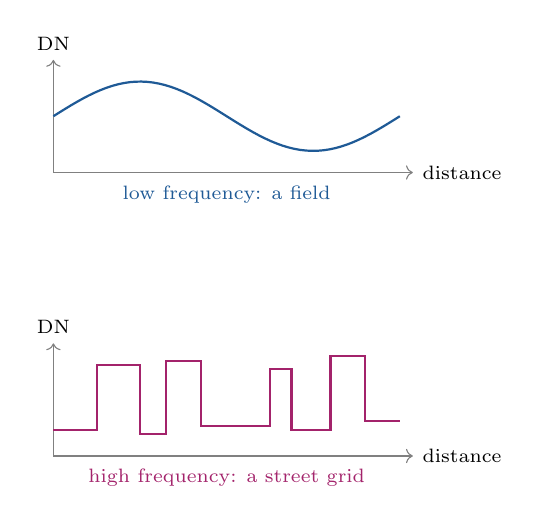
\begin{tikzpicture}[x=0.55cm, y=0.55cm]
\draw[->, gray] (0,0) -- (8.3,0) node[right, black]{\scriptsize distance};
\draw[->, gray] (0,0) -- (0,2.6) node[above, black]{\scriptsize DN};
\draw[thick, lpcol, domain=0:8, samples=60] plot (\x, {1.3 + 0.8*sin(\x*45)});
\node[lpcol, font=\scriptsize] at (4,-0.5) {low frequency: a field};
\begin{scope}[yshift=-3.6cm]
\draw[->, gray] (0,0) -- (8.3,0) node[right, black]{\scriptsize distance};
\draw[->, gray] (0,0) -- (0,2.6) node[above, black]{\scriptsize DN};
\draw[thick, hpcol] (0,0.6) -- (1,0.6) -- (1,2.1) -- (2,2.1) -- (2,0.5) -- (2.6,0.5) -- (2.6,2.2)
  -- (3.4,2.2) -- (3.4,0.7) -- (5,0.7) -- (5,2.0) -- (5.5,2.0) -- (5.5,0.6) -- (6.4,0.6)
  -- (6.4,2.3) -- (7.2,2.3) -- (7.2,0.8) -- (8,0.8);
\node[hpcol, font=\scriptsize] at (4,-0.5) {high frequency: a street grid};
\end{scope}
\end{tikzpicture}
\end{columns}
\end{frame}
\note{[Sangeeta | 0:30 | 1:00]\\
A satellite image is a grid of numbers. Spatial frequency is the number of changes in brightness per unit distance. Over a field or a lake the values change slowly; that is low frequency. Across a street grid or a ridge crest they jump every few pixels; that is high frequency. Any image can be thought of as a broad pattern plus a layer of edges and texture, and a filter lets us keep one and suppress the other.}

\begin{frame}{Low-pass flattens edges; high-pass and high-boost sharpen them}
\begin{columns}[T]
\column{0.32\textwidth}
\small
\textcolor{lpcol}{\textbf{Low-pass (LPF)}}\\ averages neighbours\\ $\Rightarrow$ smoothing, less noise

\medskip
\textcolor{hpcol}{\textbf{High-pass (HPF)}}\\ HPF = original $-$ LPF\\ $\Rightarrow$ only edges remain

\medskip
\textbf{High-boost}\\ original $+\;k\cdot$HPF\\ $\Rightarrow$ sharper, colours kept
\column{0.66\textwidth}
\adjincludegraphics[trim={{0.27\width} 0 0 0}, clip, width=0.95\textwidth]{fig06_line_profile.png}
\source{NIR reflectance along a 1.6 km line across a cleared patch on the ridge (report Fig.\ 1.1).}
\end{columns}
\takeaway{\small Both can be computed in the \emph{spatial} domain (kernels) or the \emph{frequency} domain (FFT masks).}
\end{frame}
\note{[Sangeeta | 0:35 | 1:35]\\
A low-pass filter replaces each pixel by an average of its neighbours, so the image becomes smoother. A high-pass filter keeps only the abrupt changes; the classic remote sensing form is the original minus a smoothed copy. Adding a fraction of that edge layer back gives a high-boost image. The plot is real data along one line on the ridge. The black line is the original. The blue low-pass curves are flatter, and the pink high-boost curves are steeper and overshoot at every edge. Both families can be computed in two ways, which Pranay will explain.}

\begin{frame}{Aim: decide which filter is most suitable, application by application}
\small
Smoothing and edge enhancement do opposite jobs, so we split the brief into five questions:
\medskip

\begin{tabular}{@{}cl@{}}
\toprule
Experiment & Question \\
\midrule
E1 & Which filter removes noise best? \\
E2 & Which filter helps automatic land-cover classification most? \\
E3 & Which filter makes edges, boundaries and lineaments clearest? \\
E4 & How much does each filter change the reflectance values? \\
E5 & Is the spatial or the frequency route faster? \\
\bottomrule
\end{tabular}

\takeaway{\small The answers are combined in a \textbf{decision matrix}: one best filter per application.}
\end{frame}
\note{[Sangeeta | 0:25 | 2:00]\\
Since smoothing and sharpening are meant for different jobs, asking for one best filter would not make sense. So we split the question into five, each answered by one experiment: noise removal, classification, edges, change to the spectra, and speed. At the end the five answers are combined in a decision matrix. Sangam will now describe the area and the data.}

% ================================================================== 2 Study area and data (Sangam)
\speaker{Sangam}
\section{Study Area and Data}

\begin{frame}{The Aravalli ridge holds ridges, city and farmland in one scene}
\centering
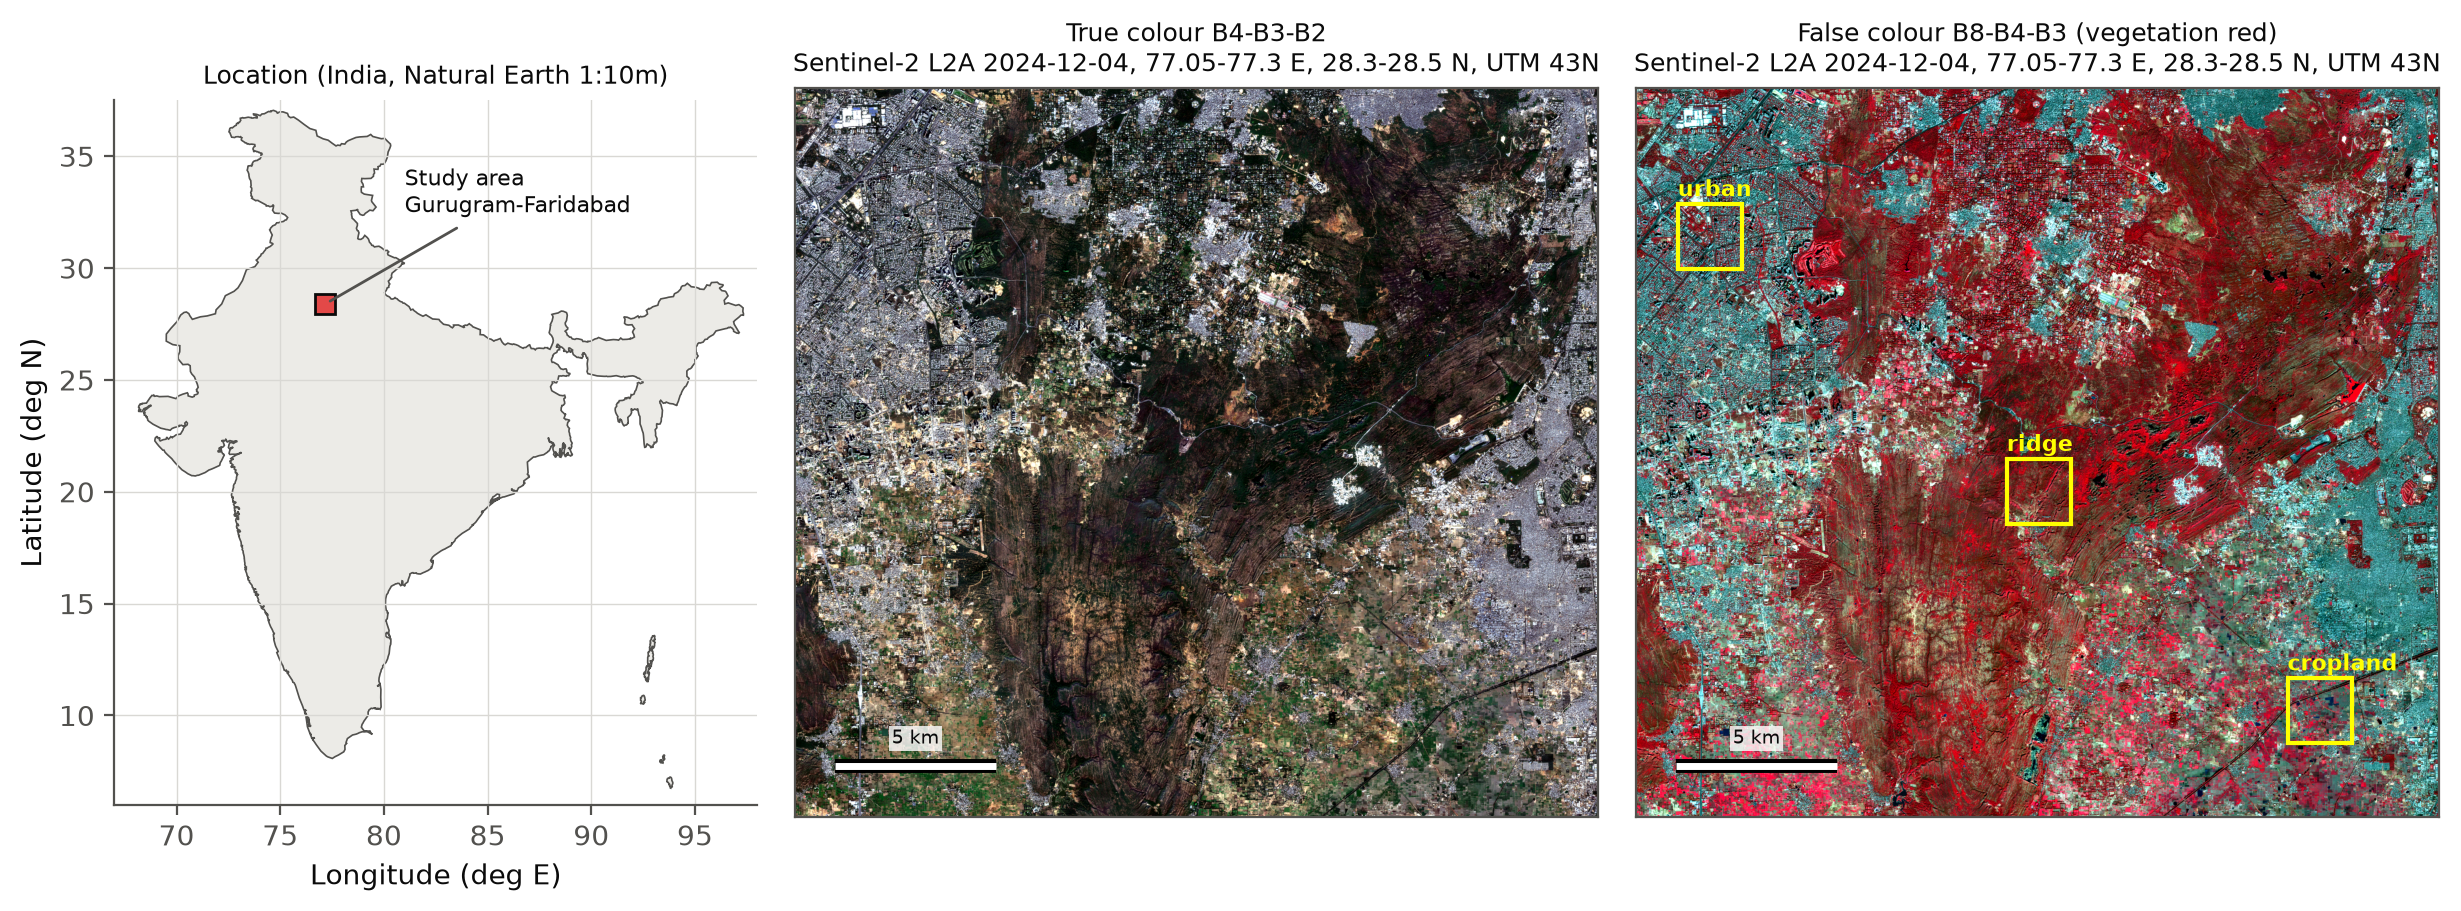
\includegraphics[width=0.86\textwidth]{fig01_study_area.png}
\source{Left: location. Centre: true colour. Right: false colour (NIR, red, green), vegetation red. Yellow boxes: ridge, urban and cropland windows.}

\vspace{3pt}
\scriptsize
\begin{tabular}{@{}ll@{}}
\textbf{Area}: 77.05--77.30$^\circ$E, 28.30--28.50$^\circ$N, 25 $\times$ 23 km &
\textbf{High frequency}: folded quartzite ridges, Gurugram streets \\
\textbf{Low frequency}: crop parcels in the south-east &
\textbf{Also}: old quarries, a few ponds \\
\end{tabular}
\end{frame}
\note{[Sangam | 0:40 | 2:40]\\
Our study area is a 25 by 23 kilometre box over the Aravalli ridge between Gurugram and Faridabad. We chose it because one scene holds very different textures. The folded quartzite ridges have long parallel linear features, and Gurugram has a dense street grid; both are high frequency and test the high-pass filters. The crop parcels in the south-east are smooth and test the low-pass filters. The three yellow boxes are two kilometre windows that we use for all zoomed comparisons later.}

\begin{frame}{Scenes were ranked by cloud and haze inside the study area}
\begin{columns}[T]
\column{0.55\textwidth}
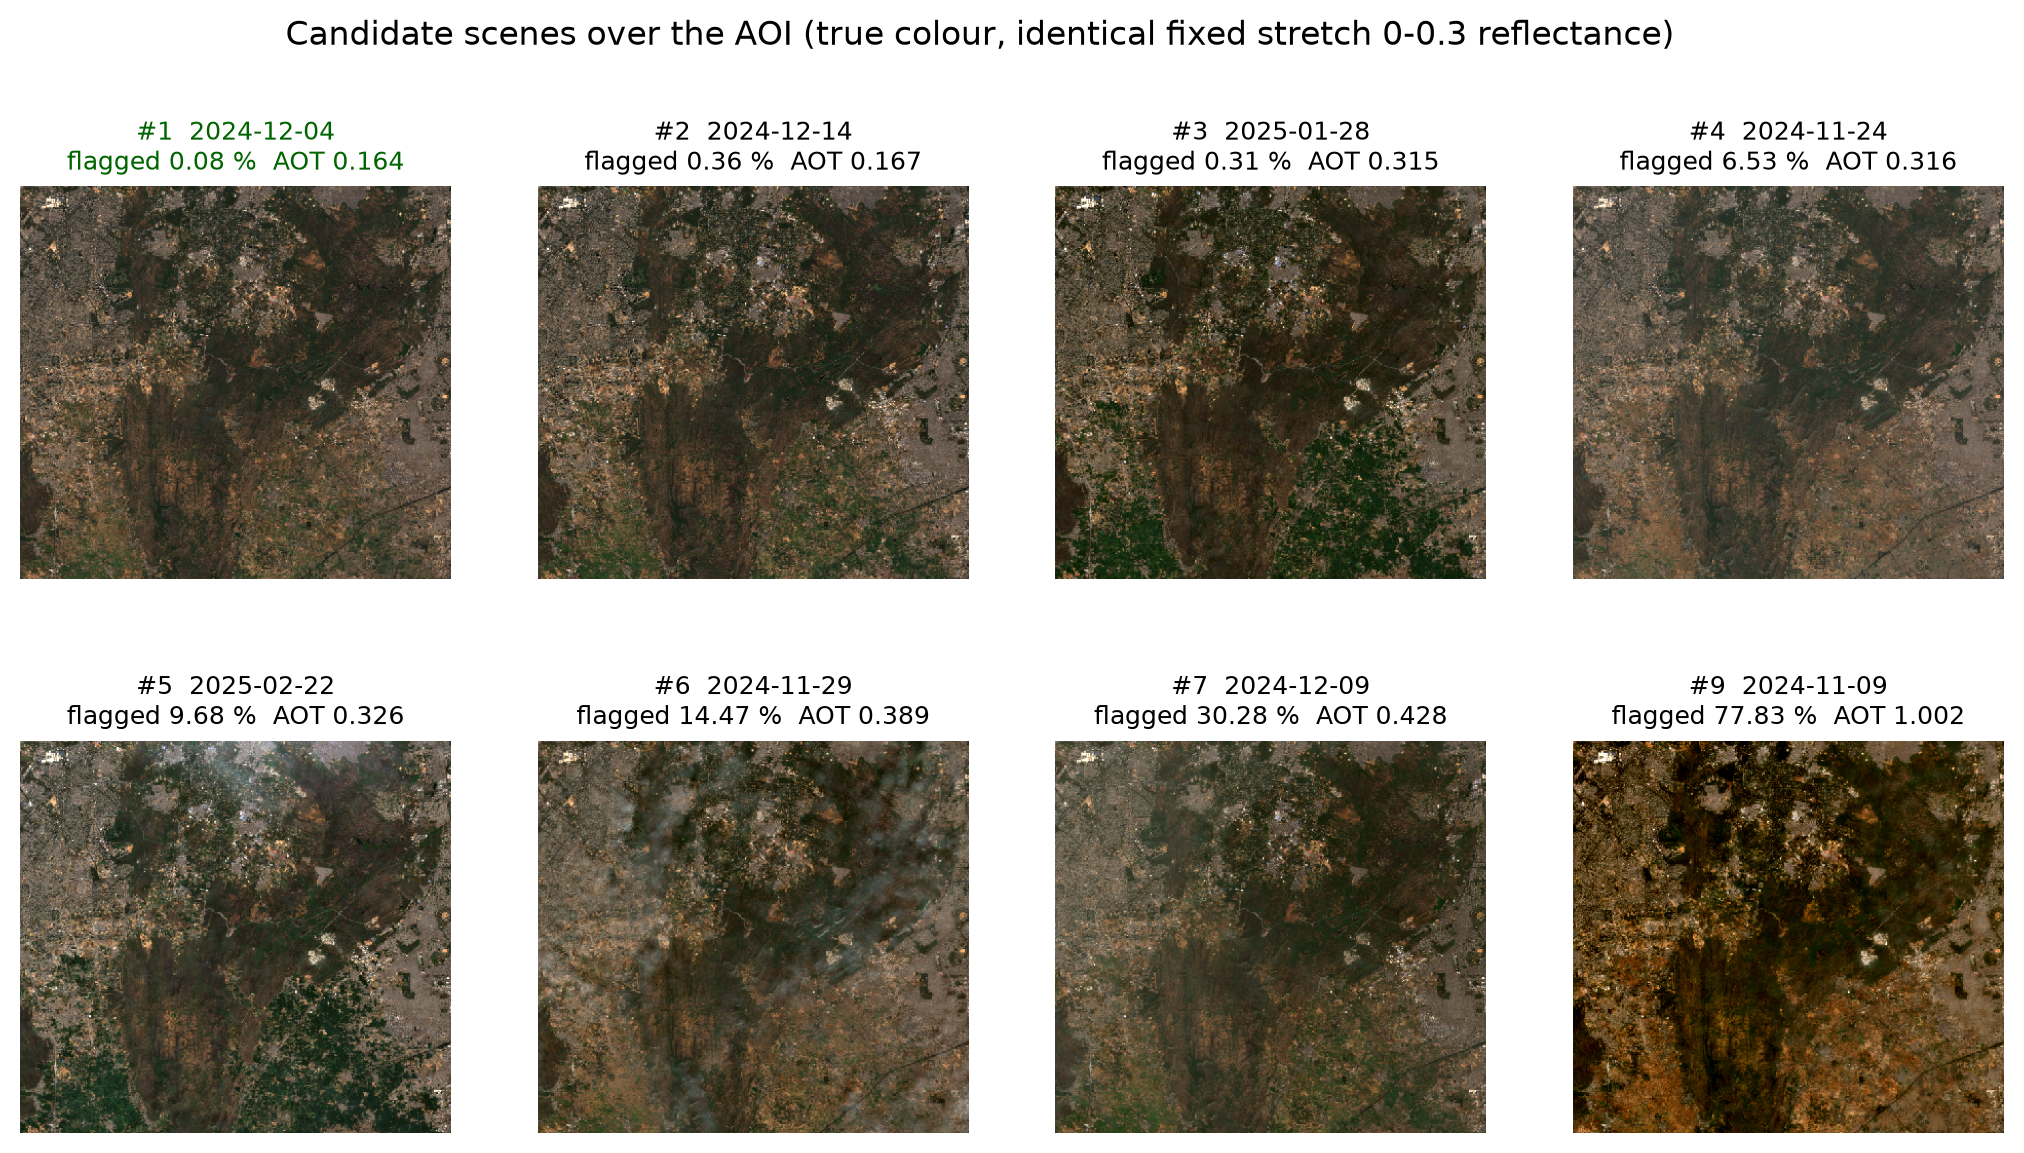
\includegraphics[width=\textwidth]{scene_candidates.png}
\source{Candidate scenes over the study area, same colour stretch; flagged share and mean AOT above each.}
\column{0.43\textwidth}
\footnotesize
\begin{itemize}
\item Sentinel-2 Level-2A \citep{drusch2012}, Google Earth Engine
\item Nov 2024 -- Feb 2025, scene cloud $<5\%$: <<n_candidates>> scenes
\item Flagged pixels \emph{inside the box}: <<bad_min>>\% to <<bad_max>>\%
\item Ranked by scene classification, s2cloudless and aerosol optical thickness (AOT)
\end{itemize}
\smallskip
\begin{tabular}{@{}ll@{}}
\toprule
Chosen scene & <<acq_date>>, tile <<tile>> \\
Flagged pixels & <<bad_pct>>\%, AOT <<aot>> \\
Bands & B2, B3, B4, B8 at 10 m \\
Grid & <<width>> $\times$ <<height>> px, UTM 43N \\
Reflectance & DN / 10000, clipped to [0, 1] \\
\bottomrule
\end{tabular}
\end{columns}
\end{frame}
\note{[Sangam | 0:50 | 3:30]\\
We used Sentinel-2 Level-2A surface reflectance from Google Earth Engine, with the four 10 metre bands: blue, green, red and near-infrared. Winter is usually the clearest season over Delhi, so we searched November 2024 to February 2025 for scenes under five percent cloud; <<n_candidates>> qualified. But the scene-wide cloud figure was misleading: inside our box the share of cloudy, hazy or missing pixels ranged from <<bad_min>> to <<bad_max>> percent, because winter smog is not counted as cloud. So the program scored every scene inside the box only and picked the cleanest one, from <<acq_date>>, with <<bad_pct>> percent flagged pixels. We used one real scene, not a composite, because compositing is itself a kind of smoothing.}

\begin{frame}{ESA WorldCover 2021 provides the land-cover reference}
\begin{columns}[c]
\column{0.40\textwidth}
\adjincludegraphics[trim={0 {0.13\height} {0.75\width} {0.08\height}}, clip, height=0.58\textheight]{fig07_classification_maps.png}
\column{0.56\textwidth}
\small
WorldCover v200 \citep{zanaga2022}, 10 m, regridded to the Sentinel-2 grid (nearest neighbour), classes merged:
\medskip

\footnotesize
\begin{tabular}{@{}lr@{}}
\toprule
Class & Share of area \\
\midrule
Trees & <<cls_trees>>\% \\
Shrub/Grass & <<cls_shrub>>\% \\
Cropland & <<cls_cropland>>\% \\
Built-up & <<cls_built>>\% \\
Bare/Mining & <<cls_bare>>\% \\
Water (dropped, $<0.5\%$) & <<water_pct>>\% \\
\bottomrule
\end{tabular}
\end{columns}
\takeaway{\small WorldCover is itself a classifier output: a \emph{reference map}, not ground truth.}
\end{frame}
\note{[Sangam | 0:30 | 4:00]\\
To judge classification and boundaries we needed a land-cover map. We used ESA WorldCover 2021 at 10 metres, put on the same pixel grid as our scene, and merged its classes into six groups. Water covered only <<water_pct>> percent of the area, too little to train on, so it was dropped, leaving five classes. One caution: WorldCover is itself produced by a classifier, so it is a reference, not ground truth. Pranay will now explain how the filters and experiments work.}

% ================================================================== 3 Methods (Pranay)
\speaker{Pranay}
\section{Methods}

\begin{frame}{Workflow: data, filter, test, decide}
\begin{columns}[c]
\column{0.50\textwidth}
\centering
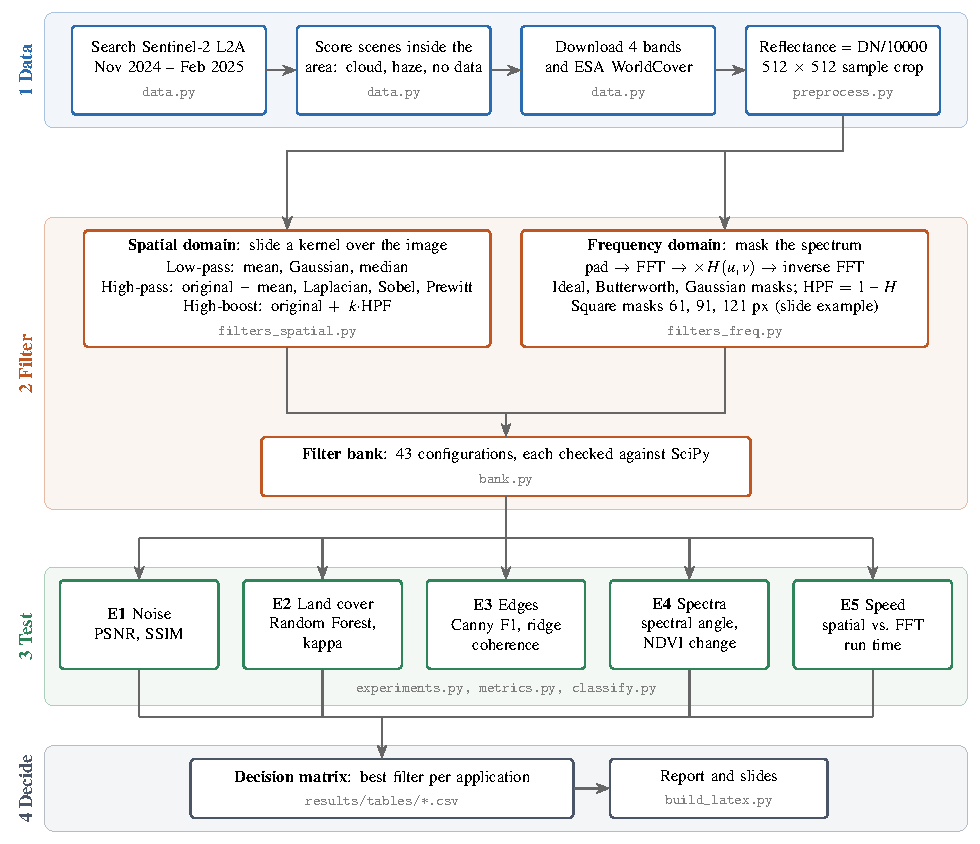
\includegraphics[height=0.76\textheight]{flowchart.pdf}
\column{0.48\textwidth}
\small
\begin{itemize}
\item Python package \texttt{rsfilter}; grey text in each box names the module
\item All filters written in NumPy, per band, on float32 reflectance
\item Unit tests against \texttt{scipy.ndimage}: max.\ difference $<10^{-5}$
\item Mirror (reflect) padding at the image border
\item One command, \texttt{python scripts/run\_all.py}, repeats everything; seed 42
\end{itemize}
\end{columns}
\end{frame}
\note{[Pranay | 0:30 | 4:30]\\
The work runs in four stages: data, filtering, testing and the decision. Every step is a function in our Python package. We wrote all filters ourselves in NumPy and used SciPy only as a reference inside unit tests; the largest disagreement is below ten to the minus five. At the border we mirror the image, so no artificial black frame enters the result. The random seed is fixed at 42 and one command reproduces every number in the report and on these slides.}

\begin{frame}{Spatial domain: each output pixel is a weighted sum of its neighbours}
\begin{equation*}
g(x,y) \;=\; \sum_{s=-a}^{a}\;\sum_{t=-b}^{b} w(s,t)\; f(x-s,\; y-t)
\end{equation*}
\small
\begin{itemize}
\item $f$: input band, $w$: kernel of size $(2a+1)\times(2b+1)$, $g$: output
\item Convolution flips the kernel by 180$^\circ$; irrelevant for our symmetric kernels
\item \textbf{Shift and accumulate}: pad once, then for every kernel cell $(s,t)$\\
\quad $g \mathrel{+}= w(s,t)\cdot$ (padded image shifted by $(s,t)$)\\
\quad $\Rightarrow$ loop over $(2a+1)(2b+1)$ cells, not over millions of pixels
\item Cost per pixel $\propto$ number of kernel cells $= n^2$ for an $n\times n$ kernel
\end{itemize}
\source{\citet{gonzalez2018}, Ch.\ 3.}
\end{frame}
\note{[Pranay | 0:40 | 5:10]\\
In the spatial domain, every output pixel g is a weighted sum of the input pixels f around it, with the weights held in a kernel w. Formally this is a convolution, which rotates the kernel by 180 degrees, but all our kernels are symmetric so that makes no difference. Instead of looping over pixels, our code loops over the kernel cells: for each cell it shifts the whole padded image, multiplies by the weight and adds it to the output. This is memory-light and easy to verify. Note the cost grows with n squared; that matters for the run-time experiment.}

\begin{frame}{Spatial kernels: low-pass averages, high-pass differences}
\footnotesize
\begin{columns}[T]
\column{0.47\textwidth}
\begin{block}{Low-pass}
Mean: $\;w_{\text{mean},3} = \tfrac{1}{9}\begin{bmatrix}1&1&1\\1&1&1\\1&1&1\end{bmatrix}$, $n=3,5,7,9$

\medskip
Gaussian: $\;w(s,t)\propto \exp\!\big(-\tfrac{s^2+t^2}{2\sigma^2}\big)$\\
side $2\lceil 3\sigma\rceil+1$, $\sum w = 1$, $\sigma=1,2,3$

\medskip
Median ($n=3,5$): median of the window;\\
non-linear, ignores single extreme values
\end{block}
\column{0.51\textwidth}
\begin{block}{High-pass}
$\text{HPF}_n = f - \text{mean}_{n\times n}(f)$ \hfill \citep{lillesand2015}

\medskip
$w_{\text{Lap},4}=\begin{bmatrix}0&1&0\\1&-4&1\\0&1&0\end{bmatrix}\;
w_{\text{Sobel},x}=\begin{bmatrix}-1&0&1\\-2&0&2\\-1&0&1\end{bmatrix}$

\medskip
Gradient magnitude $\sqrt{G_x^2+G_y^2}$ ($G_y$: transposed kernel); Prewitt uses weights 1, 1, 1

\medskip
High-boost: $\;\text{enhanced} = f + k\cdot\text{HPF}_n$,\; $k = 0.5, 1, 1.5$
\end{block}
\end{columns}
\end{frame}
\note{[Pranay | 0:50 | 6:00]\\
On the left, the low-pass kernels. The mean filter gives equal weights. The Gaussian gives nearby pixels more weight; its size is two times the ceiling of three sigma plus one, and the weights sum to one so brightness is preserved. The median is not a weighted sum at all: it takes the median of the window, so a single spike is simply ignored. On the right, the high-pass side. The remote sensing HPF is the image minus its mean filter. The Laplacian is a second derivative and responds to any change in slope. Sobel and Prewitt estimate the first derivative in x and y and we take the gradient magnitude. High-boost adds k times the HPF back to the image.}

\begin{frame}{Frequency domain: filtering becomes a multiplication of the spectrum}
\begin{columns}[T]
\column{0.52\textwidth}
\small
\[ g = \mathcal{F}^{-1}\big\{ H(u,v)\cdot\mathcal{F}\{f\}\big\} \]
\footnotesize
Pipeline per band: mirror-pad 64 px $\to$ FFT $\to$ shift centre $\to\times H\to$ shift back $\to$ inverse FFT $\to$ real part $\to$ crop.

\medskip
$D$: distance from spectrum centre, $D=1$ at Nyquist; cutoff $D_0 = 0.1, 0.2, 0.3$
\[
\begin{array}{ll}
\text{Ideal:} & H = 1 \text{ if } D\le D_0, \text{ else } 0\\[2pt]
\text{Butterworth } (n=2): & H = 1/\big(1+(D/D_0)^{4}\big)\\[2pt]
\text{Gaussian:} & H = \exp\!\big(-D^2/2D_0^2\big)\\[2pt]
\text{High-pass:} & H_{\text{HP}} = 1 - H
\end{array}
\]
Gaussian mask $\equiv$ spatial Gaussian with $\sigma = 1/(\pi D_0)$ px
\column{0.46\textwidth}
\adjincludegraphics[trim={0 0 0 {0.50\height}}, clip, width=\textwidth]{fig03_fft_spectra.png}
\source{Log-magnitude spectra of the NIR crop: original, Gaussian LPF and HPF ($D_0=0.1$).}

\smallskip
\footnotesize A sharp cut in $H$ $\Rightarrow$ a sinc-like kernel with negative side lobes $\Rightarrow$ ripples (\emph{ringing}, Gibbs, $\approx 9\%$ overshoot).
\end{columns}
\end{frame}
\note{[Pranay | 0:55 | 6:55]\\
In the frequency domain the convolution theorem turns filtering into a multiplication: Fourier transform, multiply by a mask H, transform back. We mirror-pad first because the FFT treats the image as periodic, and without padding the left edge would leak into the right. D is the distance from the centre of the spectrum, scaled so that D equals one at the Nyquist frequency. The ideal mask is a hard cut, Butterworth is a smooth roll-off, Gaussian is smoother still, and every high-pass mask is one minus the low-pass one. A Gaussian mask with cutoff D0 is the same filter as a spatial Gaussian with sigma one over pi D0, which gives us a check between the two domains. Finally, a hard cut in frequency corresponds to a sinc-shaped kernel in space, whose negative side lobes cause ripples next to edges; theory predicts about nine percent overshoot.}

\begin{frame}{Filter bank: <<n_filters>> configurations compared}
\centering
\footnotesize
\begin{tabular}{@{}lp{5.2cm}p{4.6cm}@{}}
\toprule
Family & Filter & Parameters \\
\midrule
Low-pass, spatial & Mean; Gaussian; Median & $n=3,5,7,9$; $\sigma=1,2,3$; $n=3,5$ \\
Low-pass, frequency & Ideal, Butterworth, Gaussian & $D_0 = 0.1, 0.2, 0.3$ \\
High-pass, spatial & Original $-$ mean; Laplacian; Sobel, Prewitt & $n=3,5,7$; 4-, 8-neighbour \\
High-pass, frequency & Ideal, Butterworth, Gaussian & $1-H$, $D_0 = 0.1, 0.2, 0.3$ \\
High-boost & $f + k\cdot\text{HPF}_n$ & $n=3,5,7$; $k=0.5,1.0,1.5$ \\
\bottomrule
\end{tabular}

\medskip
\footnotesize Plus the course-slide example: square ideal low-pass masks of 61, 91 and 121 px on a 512 $\times$ 512 crop.
\end{frame}
\note{[Pranay | 0:15 | 7:10]\\
Together these give <<n_filters>> configurations, covering both families in both domains. We also reproduced the example in the course slides with square ideal masks of 61, 91 and 121 pixels.}

\begin{frame}{Five experiments, each with a measure that decides the winner}
\footnotesize
\begin{tabular}{@{}lp{5.6cm}p{6.6cm}@{}}
\toprule
 & Set-up & Measure \\
\midrule
E1 & Gaussian noise $\sigma=0.02$ or 2\% salt-and-pepper on a clean 512 $\times$ 512 crop; every LPF & $\text{PSNR} = 10\log_{10}(1/\text{MSE})$ dB; SSIM \citep{wang2004} \\
E2 & Random Forest \citep{breiman2001}, 200 trees, 2000 px/class; 4 bands + NDVI after filtering & $\kappa = (p_o - p_e)/(1-p_e)$; accuracy; macro-F1; salt-and-pepper index \\
E3 & NIR band & mean gradient; Canny \citep{canny1986} edge F1 vs WorldCover boundaries (2 px); ridge coherence \\
E4 & all bands & SAM $=\arccos\frac{\mathbf{x}\cdot\mathbf{y}}{|\mathbf{x}||\mathbf{y}|}$; $|\Delta\text{NDVI}|$; RMSE \\
E5 & one full band, <<e5_shape>> px & median of 5 runs, spatial vs FFT \\
\bottomrule
\end{tabular}
\end{frame}
\note{[Pranay | 0:40 | 7:50]\\
Each experiment has one deciding measure. E1 uses PSNR, ten log ten of one over the mean squared error, since reflectance runs from zero to one; three decibels more means roughly half the error. E2 uses Cohen's kappa, which is the observed agreement p o corrected for the agreement p e expected by chance. E3 uses the F1 score of Canny edges against WorldCover class boundaries, and orientation coherence on the ridge. E4 uses the spectral angle between a pixel's four-band vector before and after filtering; zero degrees means the shape of the spectrum is unchanged. E5 is plain wall-clock time.}

\begin{frame}{Two design choices that keep the evaluation honest}
\begin{columns}[T]
\column{0.48\textwidth}
\begin{block}{E2: spatially blocked split}
\small
Neighbouring pixels are near-copies, so a random pixel split inflates accuracy.

\medskip
$\Rightarrow$ 128 $\times$ 128 px blocks, 70\% train / 30\% test\\
{\footnotesize (<<n_train_pix>> training, <<n_test_pix>> test pixels)}
\end{block}
\column{0.48\textwidth}
\begin{block}{E3: orientation coherence}
\small
Structure tensor $J = G_\rho * \begin{bmatrix}g_x^2 & g_xg_y\\ g_xg_y & g_y^2\end{bmatrix}$, eigenvalues $\lambda_1\ge\lambda_2$
\[ C = \frac{\lambda_1-\lambda_2}{\lambda_1+\lambda_2}\in[0,1] \]
\footnotesize 1: parallel ridges; 0: speckle. 2 $\times$ 2 km ridge window \citep{bigun1987}.
\end{block}
\end{columns}
\takeaway{\small No published lineament map exists here, so coherence stands in for lineament quality.}
\end{frame}
\note{[Pranay | 0:30 | 8:20]\\
Two choices need explaining. First, neighbouring pixels are almost identical, so if test pixels are drawn at random each has a near-copy in the training set and accuracy looks better than it is. We cut the area into 128 pixel blocks and split the blocks 70 to 30. Second, there is no lineament map of this area, so we measure how linear the ridge window is. The structure tensor averages the outer product of the gradient; when one eigenvalue dominates, the gradients share one direction and coherence approaches one. Random speckle gives values near zero. Aparna will now show what the filters do.}

% ================================================================== 4 Results I (Aparna)
\speaker{Aparna}
\section{Results I: Filtered Images, Ringing and Noise}

\begin{frame}{Low-pass filters keep the broad ridge but blur streets and field edges}
\centering
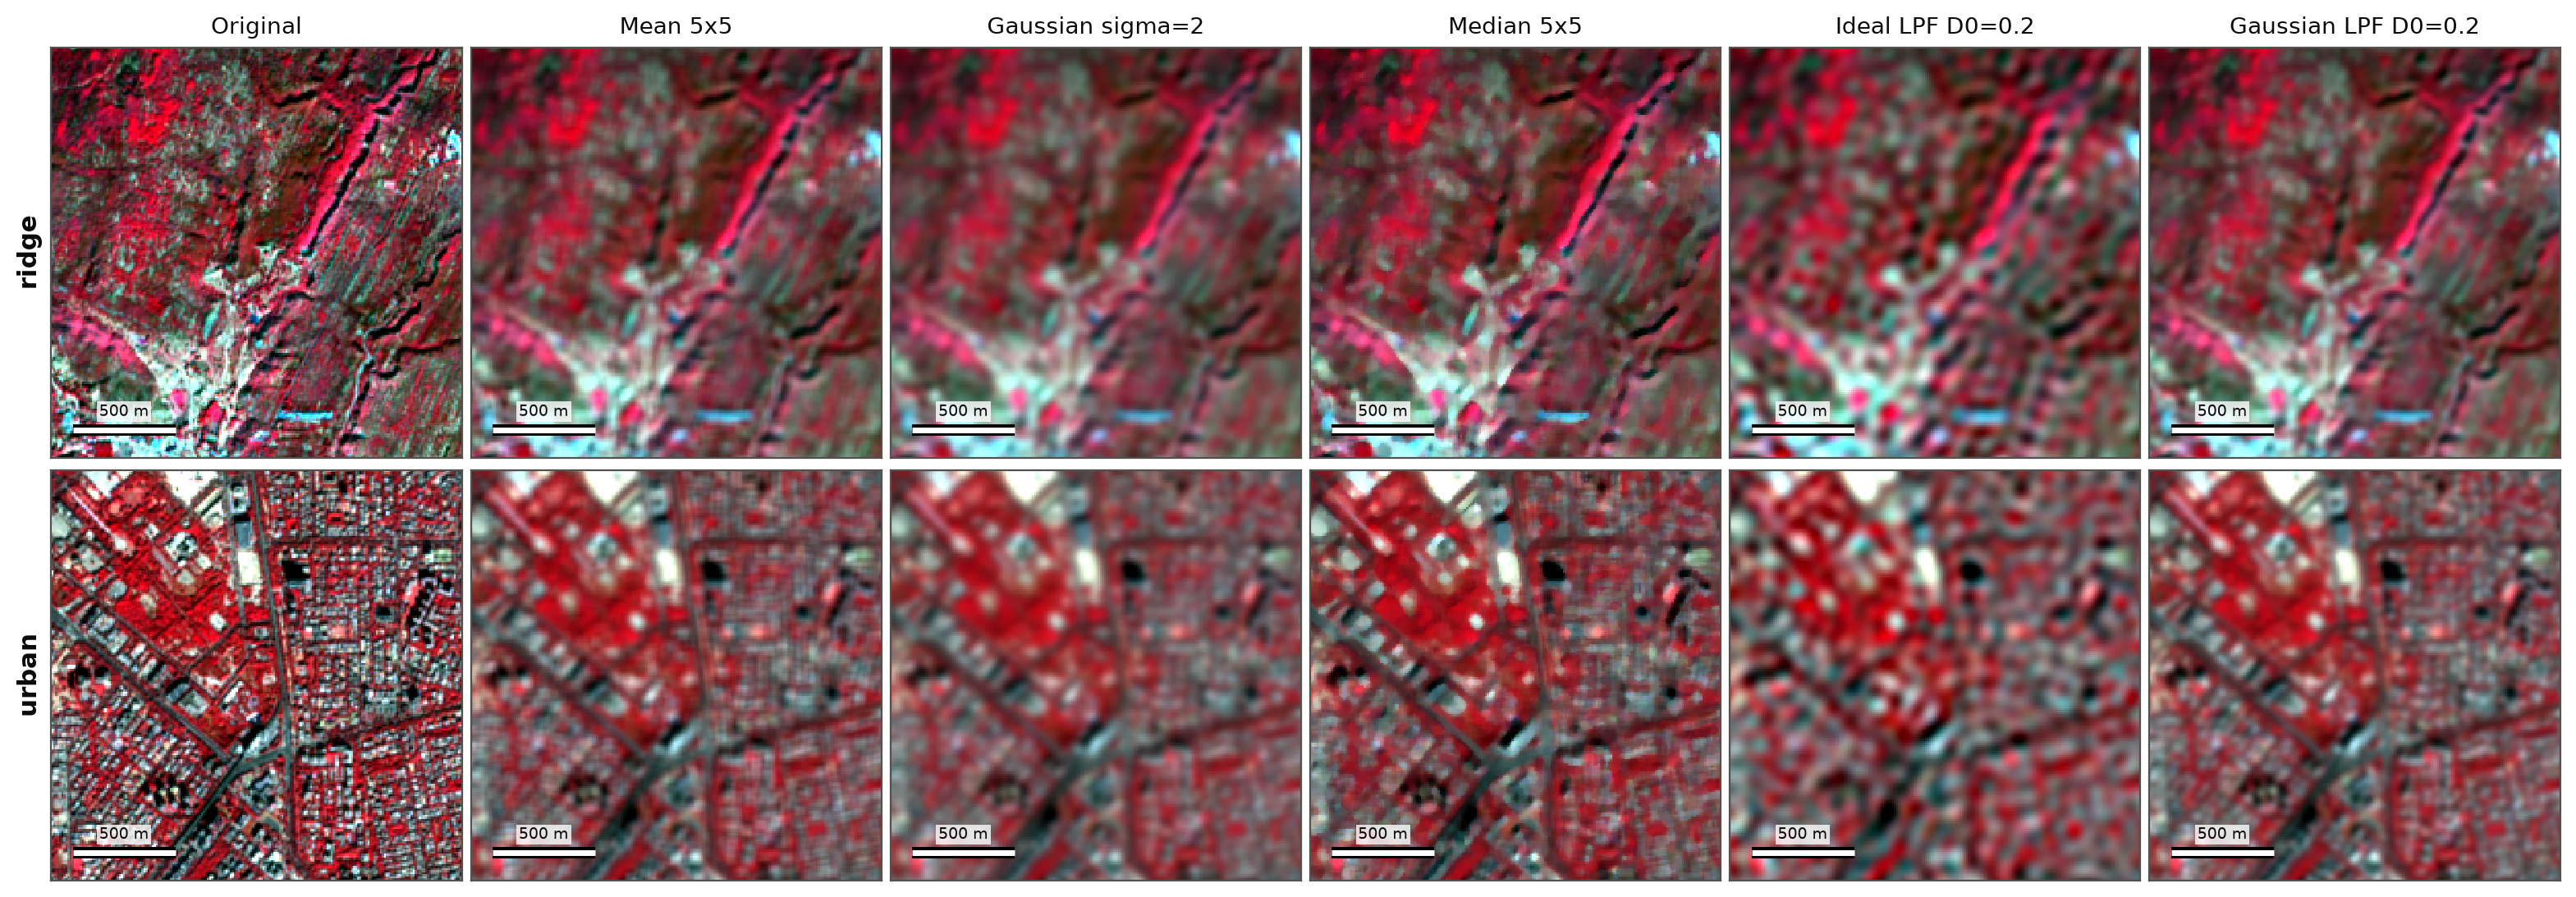
\includegraphics[width=0.97\textwidth]{slide_lpf.png}
\source{2 km windows, ridge (top) and Gurugram (bottom); false colour, same stretch in every panel.}
\takeaway{\small The median keeps straight edges sharper than a mean or Gaussian of the same size.}
\end{frame}
\note{[Aparna | 0:30 | 8:50]\\
These are two 2 kilometre windows, the ridge on top and Gurugram below, all with the same colour stretch. Every low-pass filter blurs the street grid and the field edges, while the broad shape of the ridge survives. The median keeps straight edges a little sharper, because it picks an existing value instead of averaging across the edge. The Gaussian frequency mask looks just like the spatial Gaussian, as Pranay predicted.}

\begin{frame}{High-pass filters turn flat ground grey and keep only the edges}
\centering
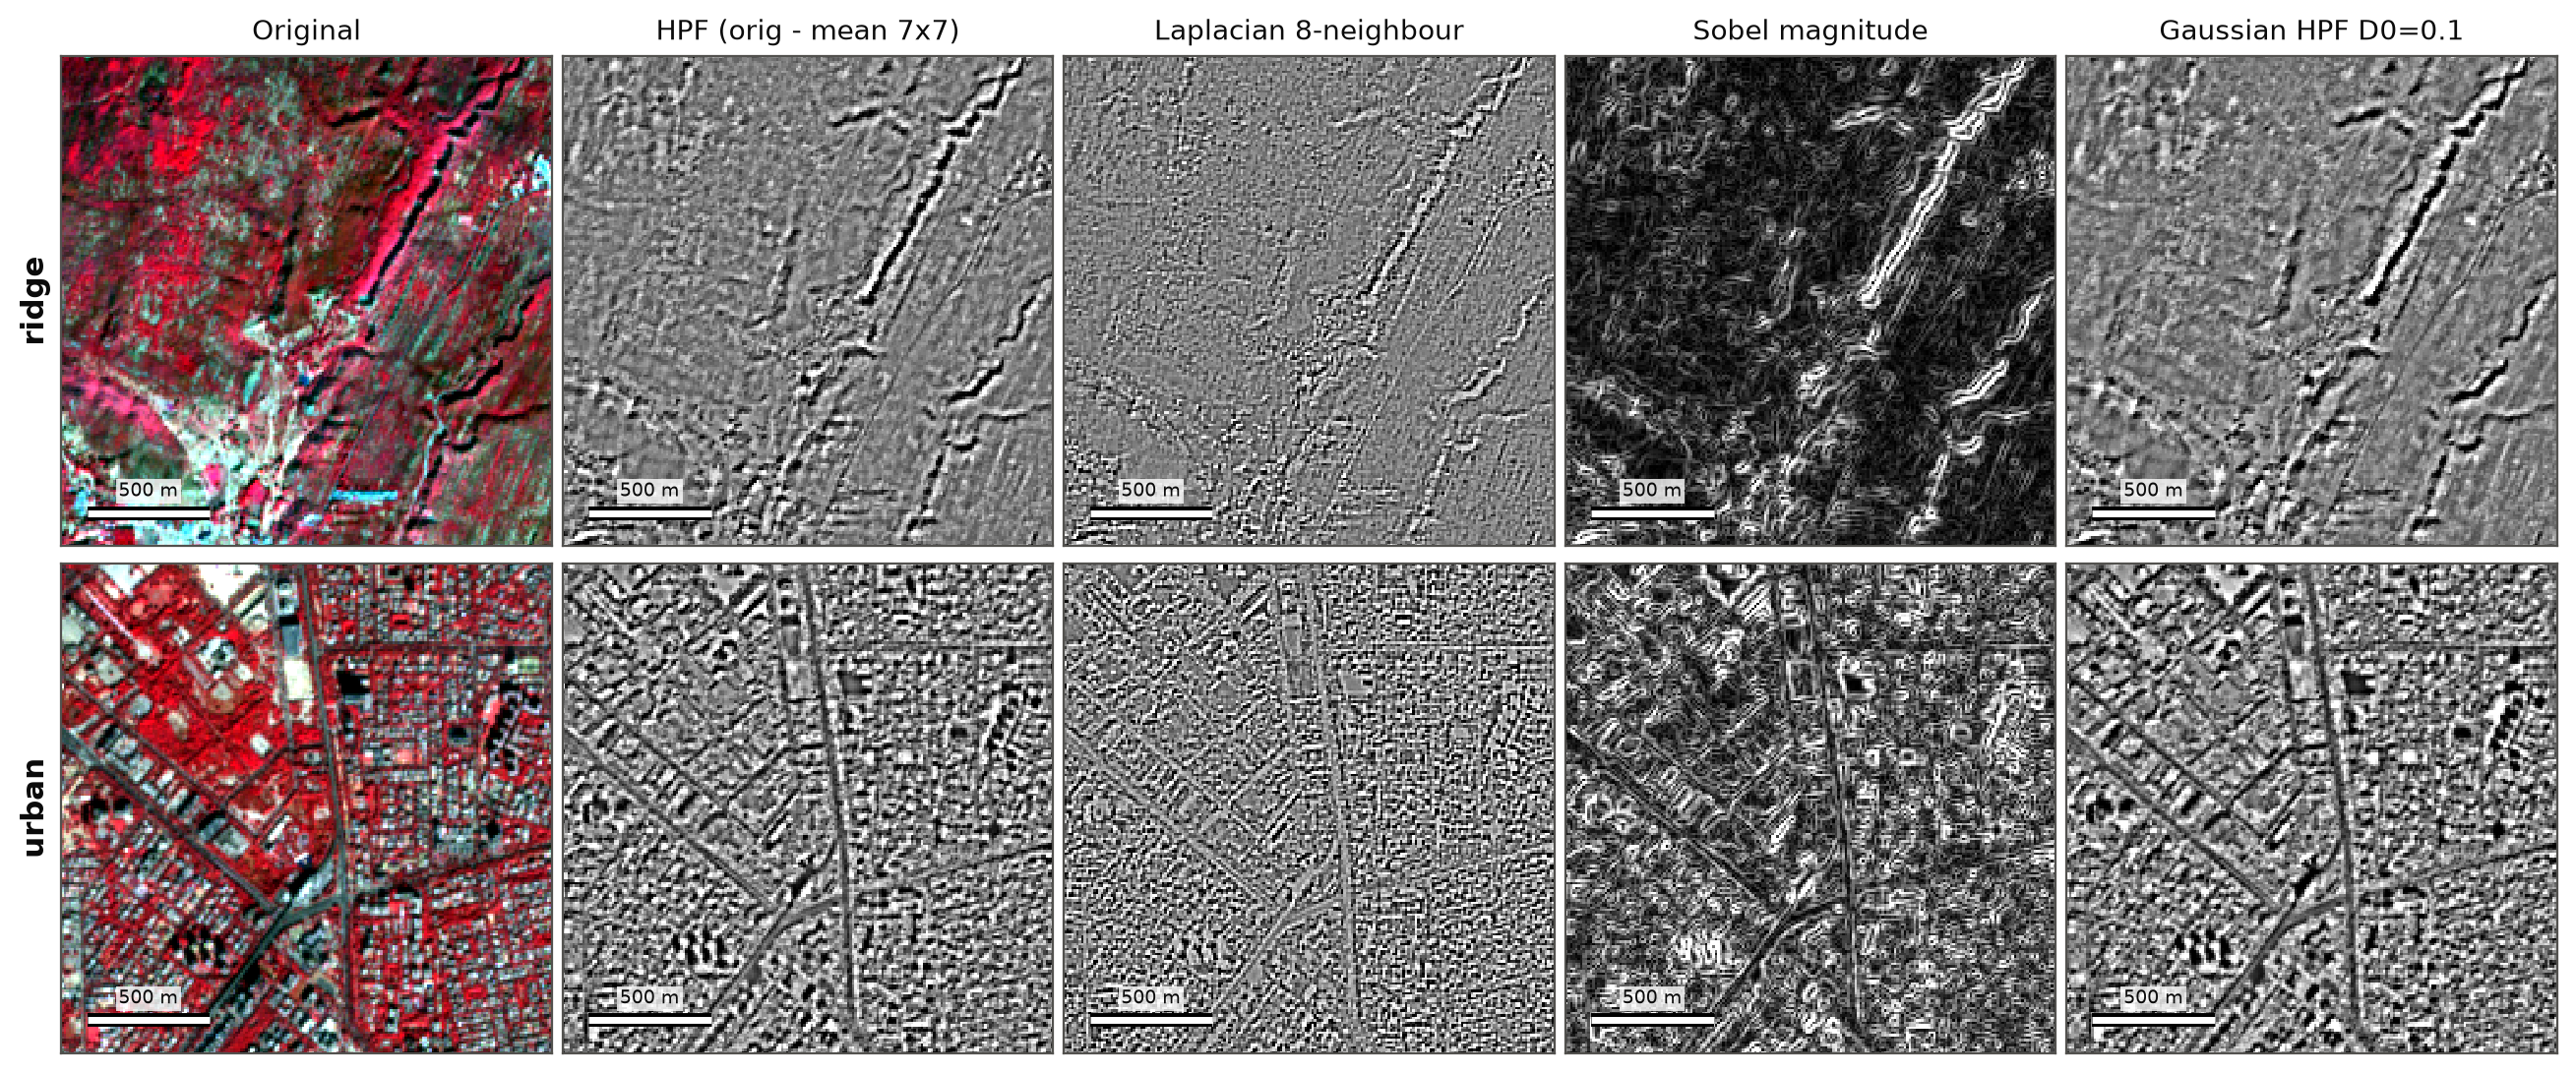
\includegraphics[width=0.93\textwidth]{slide_hpf_edges.png}
\source{NIR band, same two windows.}
\takeaway{\small $7\times7$ HPF and Sobel trace the ridge crests; the Laplacian reacts mostly to fine speckle.}
\end{frame}
\note{[Aparna | 0:25 | 9:15]\\
High-pass outputs are edge maps. Uniform ground becomes mid-grey and only the changes remain. The 7 by 7 HPF and the low-cutoff frequency HPF bring out the ridge crests, and Sobel shows edge strength in any direction. The Laplacian responds most to the finest speckle.}

\begin{frame}{High-boost sharpens boundaries and keeps the colours}
\centering
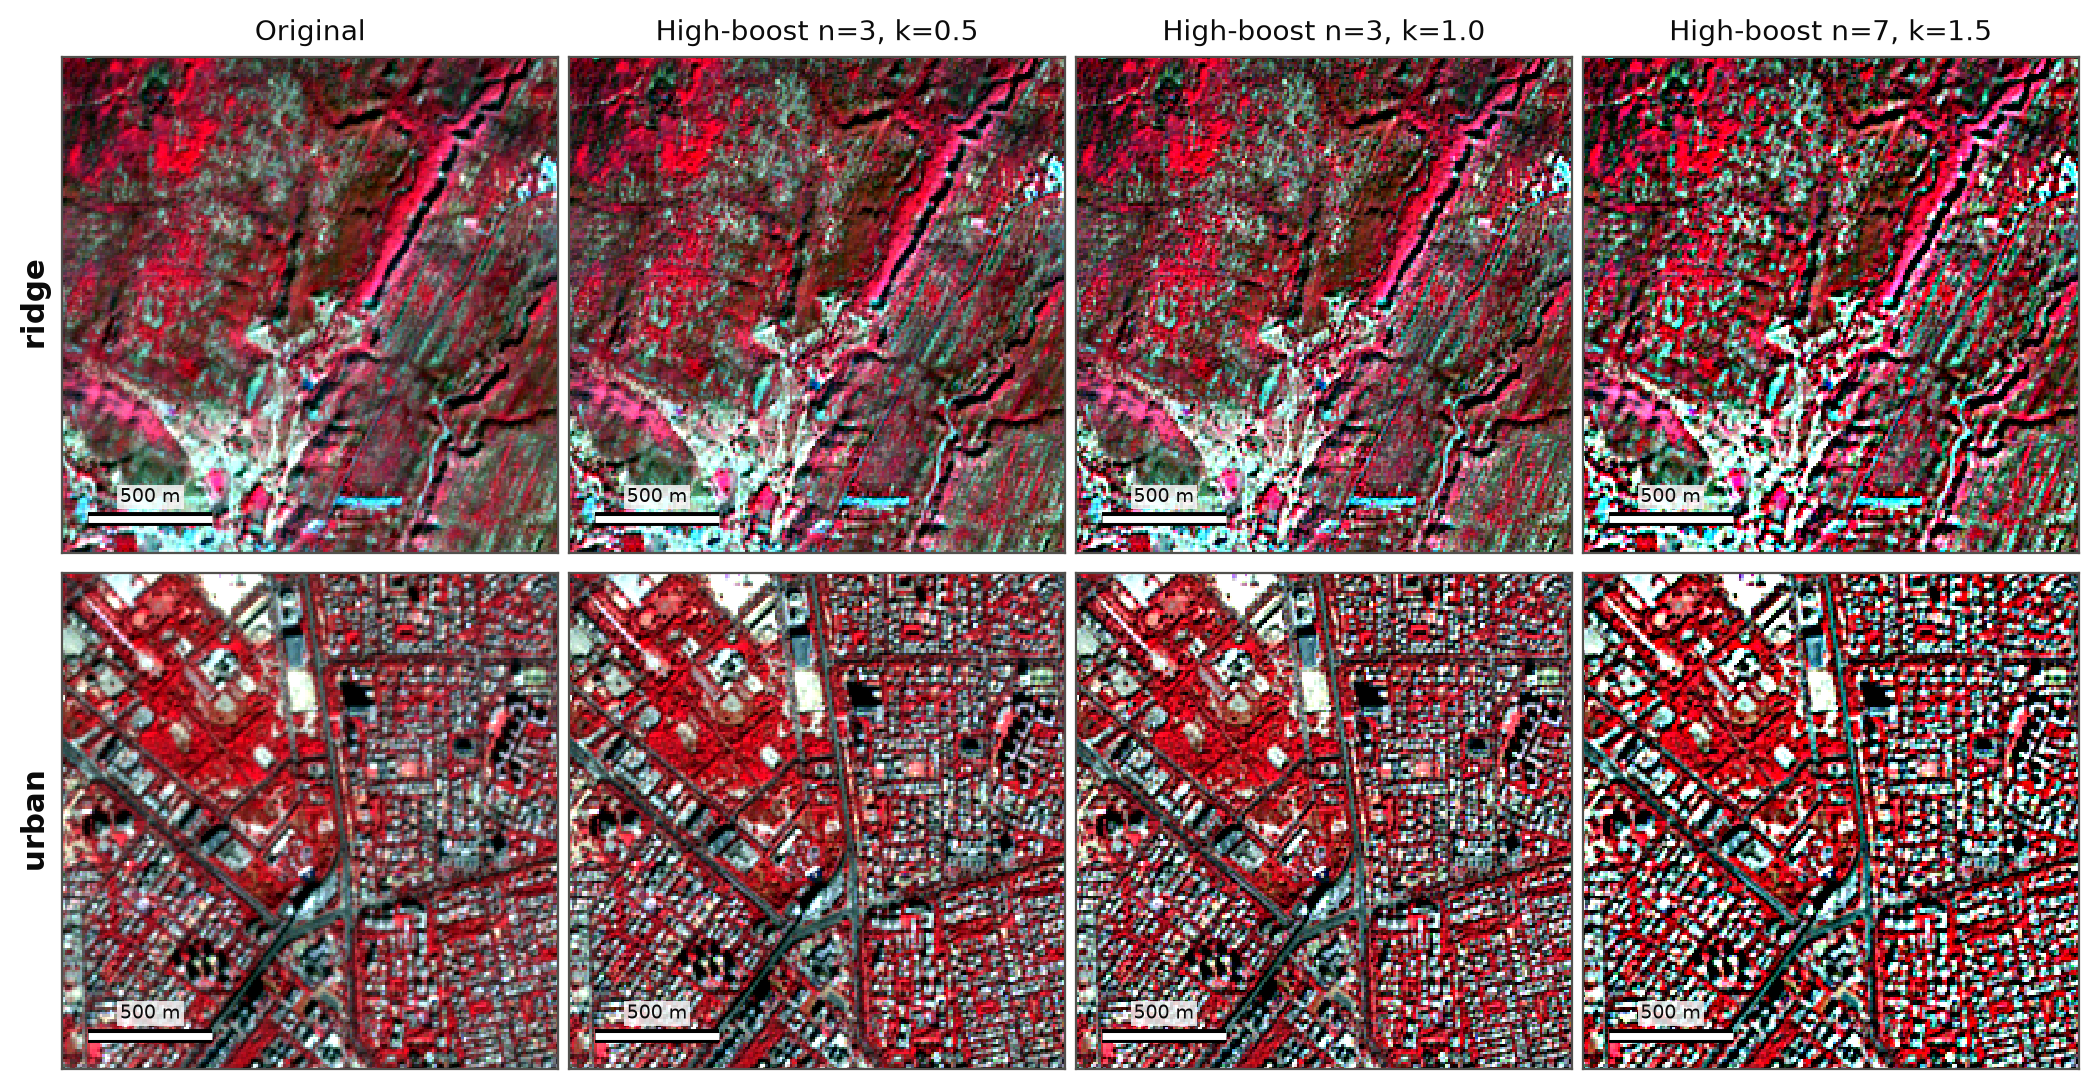
\includegraphics[height=0.66\textheight]{slide_highboost.png}
\takeaway{\small At $k=1.5$, bright and dark halos appear along roads and ridge crests.}
\end{frame}
\note{[Aparna | 0:20 | 9:35]\\
An analyst rarely looks at the bare edge layer, so here it is added back to the image. As k increases, boundaries get crisper while the colours stay the same. At k equal to 1.5 we start to see halos along roads and ridge crests, so a moderate k is better.}

\begin{frame}{The course example reproduced: smaller square mask, blurrier image}
\centering
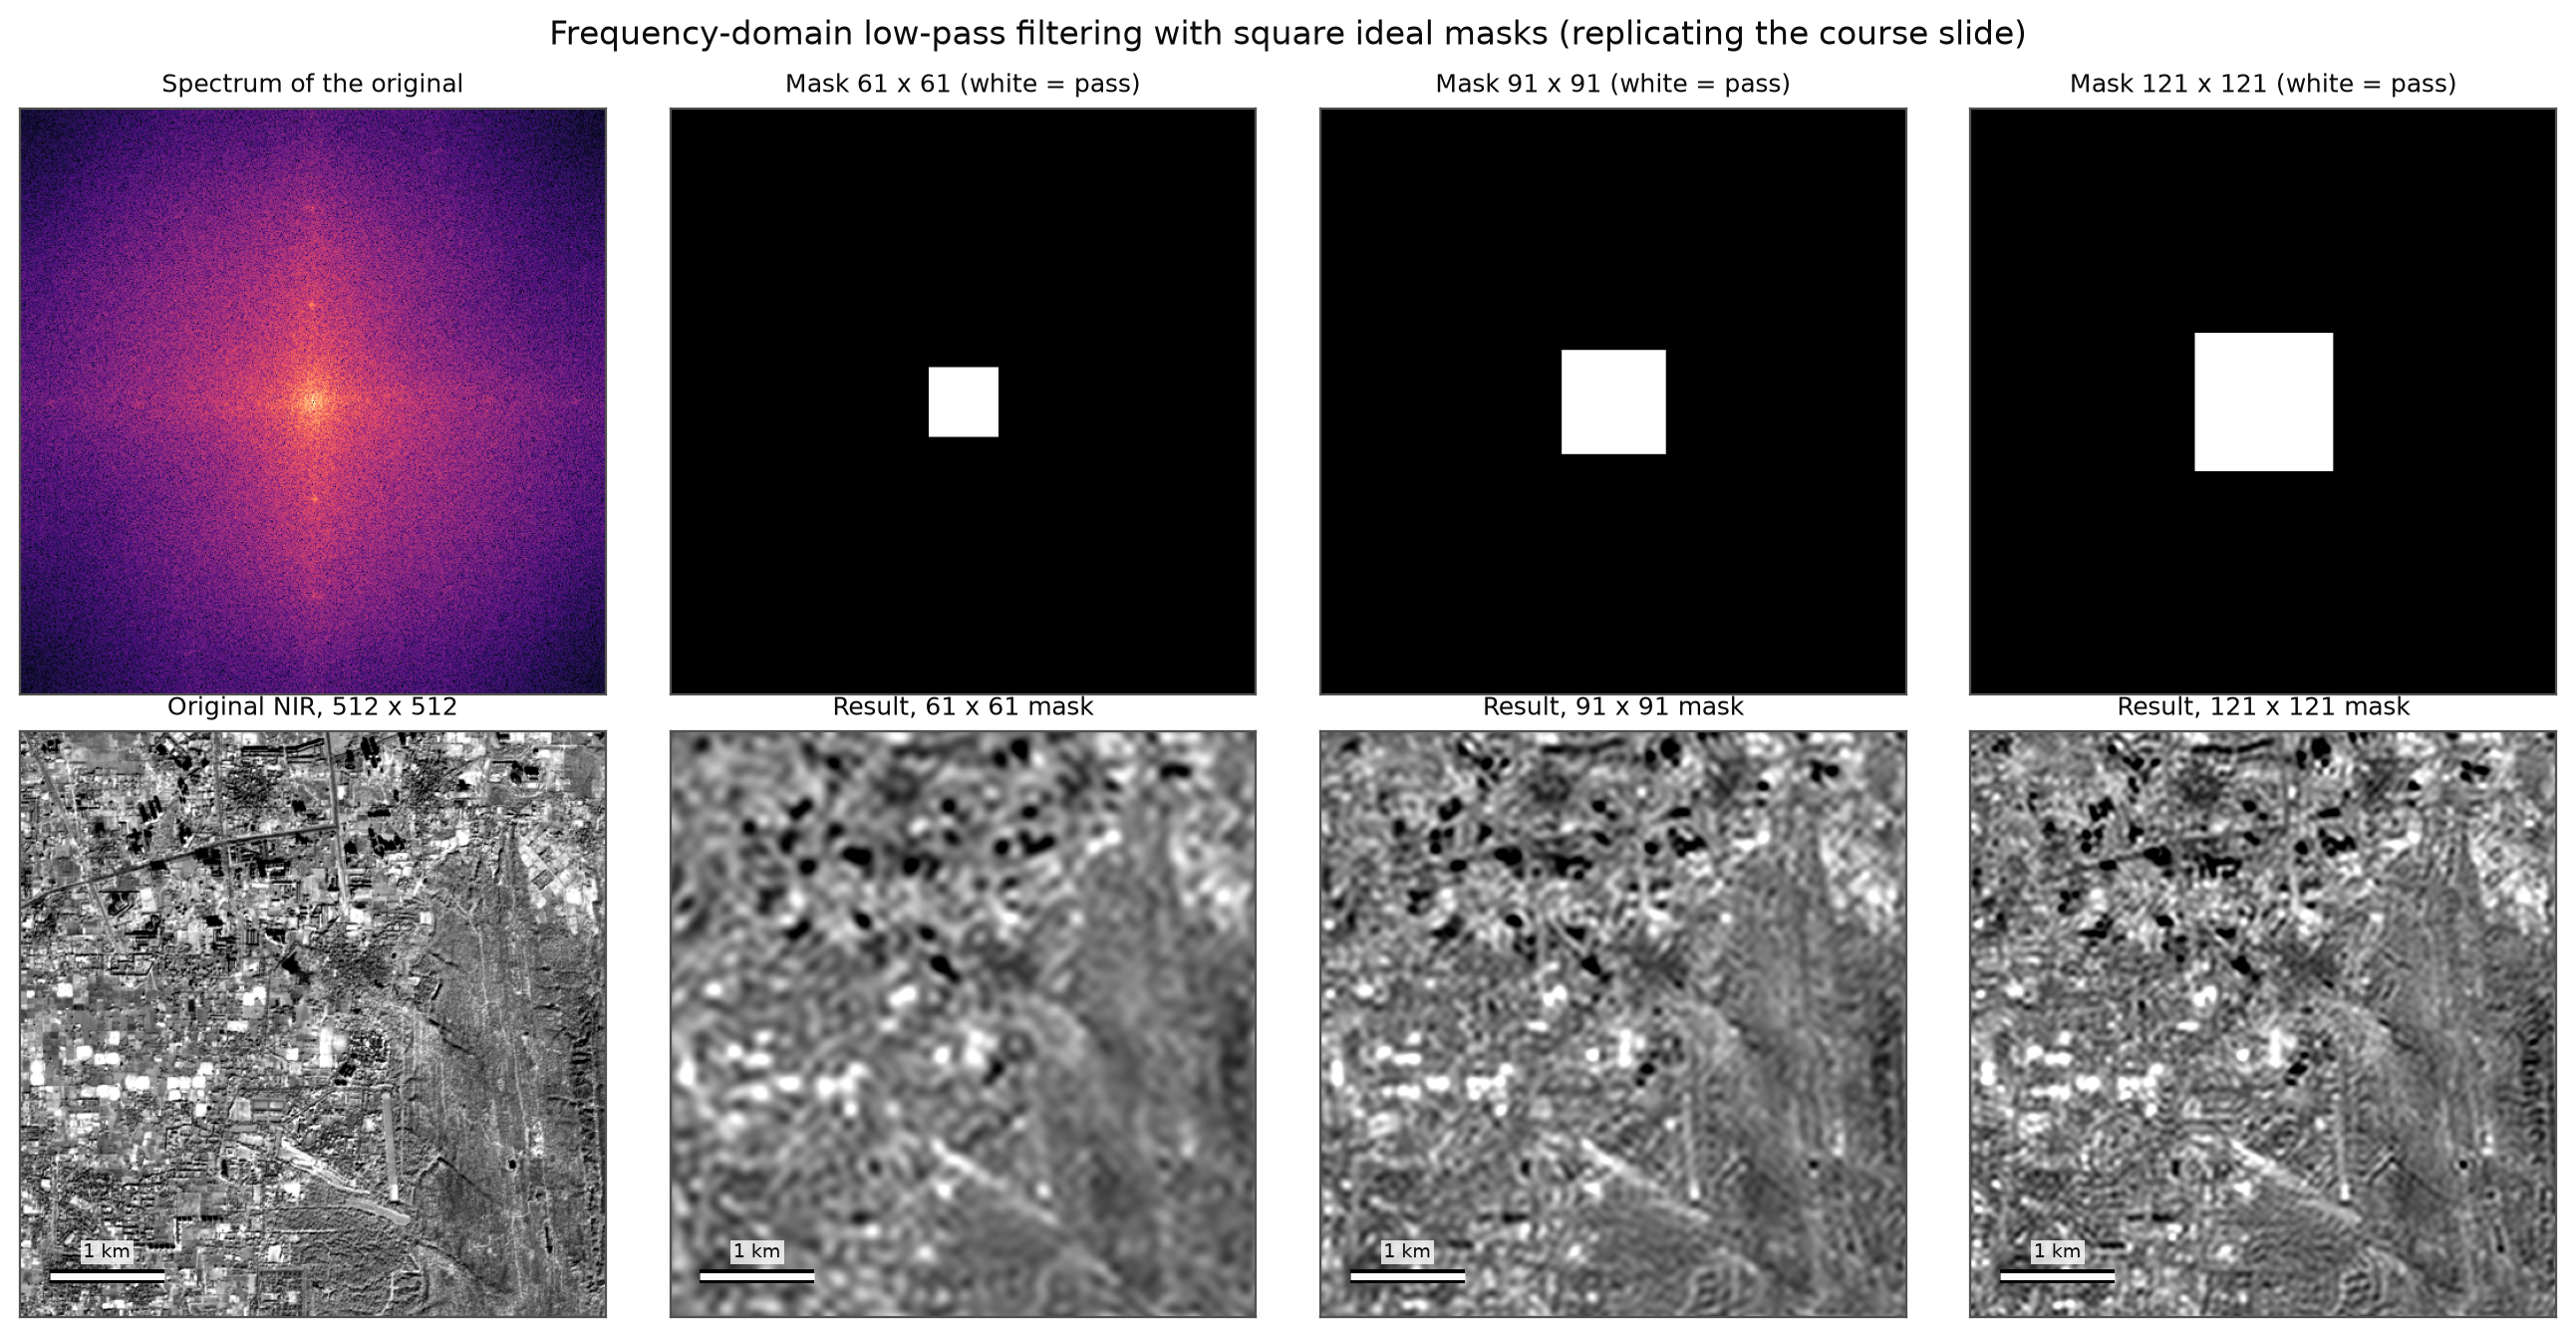
\includegraphics[height=0.66\textheight]{fig04_slide_square_masks.png}
\source{Square ideal low-pass masks of 61, 91 and 121 px (top) and the filtered NIR crop (bottom).}
\takeaway{\small All three results show a faint ripple texture.}
\end{frame}
\note{[Aparna | 0:20 | 9:55]\\
This reproduces the example from the course slides on our own crop. The top row shows the spectrum and the square masks; white means the frequency is kept. The smallest mask keeps the fewest frequencies and gives the blurriest image. All three results show a faint ripple texture, which the next slide explains.}

\begin{frame}{A sharp frequency cut causes ringing; smooth masks do not}
\centering
\adjincludegraphics[trim={0 0 0 {0.52\height}}, clip, width=0.92\textwidth]{fig05_ringing.png}
\source{The same mask code applied to a clean synthetic step edge, $D_0 = 0.1$.}

\small
\begin{tabular}{lccc}
\toprule
Mask ($D_0=0.1$) & Ideal & Butterworth & Gaussian \\
\midrule
Overshoot, \% of step height & \textbf{<<ring_ideal>>} & <<ring_butter>> & <<ring_gauss>> \\
\bottomrule
\end{tabular}
\takeaway{\small Use Gaussian or Butterworth masks, never the ideal mask.}
\end{frame}
\note{[Aparna | 0:30 | 10:25]\\
On real data the ripples are hidden by texture, so we passed a clean step edge through the same code. The ideal mask overshoots by <<ring_ideal>> percent of the step height, which matches the roughly nine percent from theory. Butterworth overshoots by <<ring_butter>> percent, and Gaussian by <<ring_gauss>>. So whenever we filter in the frequency domain we should use a smooth mask.}

\begin{frame}{E1: the best noise filter depends on the type of noise}
\begin{columns}[T]
\column{0.62\textwidth}
\scriptsize
\setlength{\tabcolsep}{3pt}
\begin{tabular}{@{}lcccc@{}}
\toprule
 & \multicolumn{2}{c}{Gaussian, $\sigma=0.02$} & \multicolumn{2}{c}{Salt-and-pepper, 2\%} \\
\cmidrule(lr){2-3}\cmidrule(l){4-5}
Filter & PSNR (dB) & SSIM & PSNR (dB) & SSIM \\
\midrule
<<e1_table>>
\bottomrule
\end{tabular}
\column{0.36\textwidth}
\small
\textbf{Random noise}: only light filters help; <<e1_g_n_worse>> of <<e1_g_n_lpf>> made it worse.

\medskip
\textbf{Impulse noise}: median $3\times3$ raises PSNR from <<e1_sp_noisy>> to <<e1_sp_best_psnr>> dB, <<e1_sp_gap>> dB ahead of the best linear filter.
\end{columns}
\takeaway{\small Median $3\times3$ for impulse noise; Gaussian $\sigma=1$ or mean $3\times3$ for random noise.}
\end{frame}
\note{[Aparna | 0:35 | 11:00]\\
For E1 we added noise to a clean crop and measured how close each filtered result came to the clean image; higher PSNR is better. With random noise the noisy image scored <<e1_g_noisy>> decibels, and only the lightest filters improved on it; <<e1_g_n_worse>> of the <<e1_g_n_lpf>> low-pass filters made it worse, because they removed more real detail than noise. With salt-and-pepper noise the 3 by 3 median was far ahead: a mean spreads each spike over its neighbours, while the median throws it away. Robin will present the remaining experiments.}

% ================================================================== 5 Results II (Robin)
\speaker{Robin}
\section{Results II: Classification, Edges and Cost}

\begin{frame}{E2: low-pass inputs classify best, high-boost inputs worst}
\centering
\footnotesize
\begin{tabular}{@{}llcccc@{}}
\toprule
Input & Family & Accuracy & $\kappa$ & Macro-F1 & Salt-and-pepper \\
\midrule
<<e2_table>>
\bottomrule
\end{tabular}
\source{Held-out blocks. Best and worst of each family; bold = best (lowest for salt-and-pepper).}
\takeaway{\small Smoothing removes within-class variation (roof types, shadows, mixed pixels) before classification.}
\end{frame}
\note{[Robin | 0:35 | 11:35]\\
In E2 a Random Forest classified the area after each filter. On the raw bands kappa was <<e2_raw_kappa>>. Every low-pass input did better; the best reached <<e2_best_kappa>>, and the spatial Gaussian was almost tied with it, which is expected because, as Pranay showed, the two are nearly the same filter. High-boost inputs did worse, at best <<e2_hb_best_kappa>>. The reason is that at 10 metres one class contains many different surfaces, like roofs and shadows. Smoothing averages that variation out; sharpening makes it larger. Adding high-pass layers next to the raw bands helped a little, kappa <<e2_stack_best_kappa>>, but less than smoothing.}

\begin{frame}{E2: smoothing also halves the speckle in the classified map}
\centering
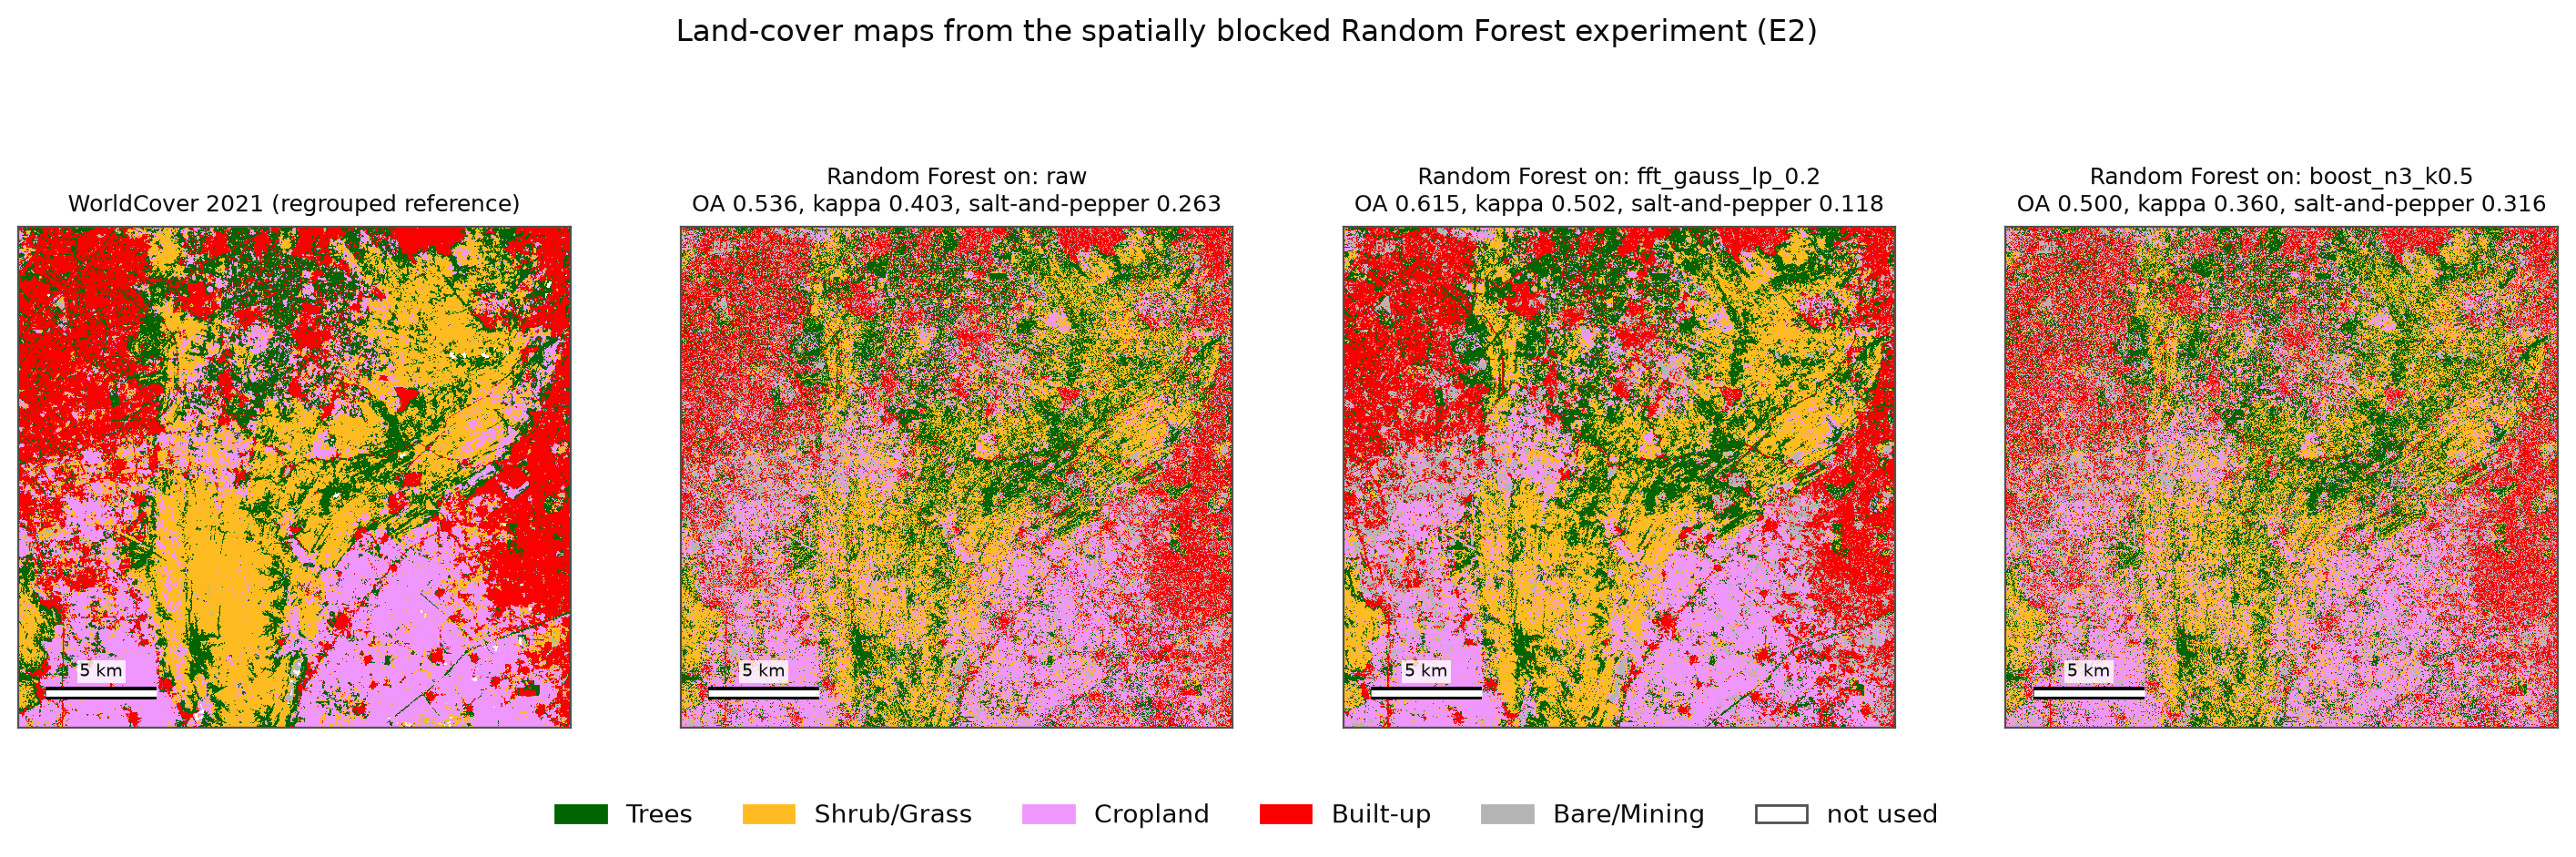
\includegraphics[width=\textwidth]{fig07_classification_maps.png}
\takeaway{\small Salt-and-pepper index: raw <<e2_raw_sp>> $\rightarrow$ best low-pass <<e2_best_sp>>.}
\end{frame}
\note{[Robin | 0:20 | 11:55]\\
Here are the maps. From the left: the WorldCover reference, the map from the raw bands, from the best low-pass input, and from the best high-boost input. The raw and high-boost maps are speckled; the low-pass map is much cleaner. The share of pixels that disagree with their neighbours fell from <<e2_raw_sp>> to <<e2_best_sp>>.}

\begin{frame}{E3: high-pass helps boundaries and ridge lineaments}
\begin{columns}[T]
\column{0.50\textwidth}
\begin{block}{Boundaries (Canny edge F1)}
\footnotesize
\begin{tabular}{@{}lc@{}}
No filter & <<e3_orig_f1>> \\
\textbf{<<p:e3_hb_best>>} & \textbf{<<e3_hb_best_f1>>} \\
Gaussian $\sigma=1$ & <<e3_g1_f1>> \\
Mean $5\times5$ & <<e3_box5_f1>> \\
\midrule
Built-up only: no filter & <<e3_bu_orig>> \\
Built-up only: best & <<e3_bu_best_f1>> \\
\end{tabular}
\end{block}
\column{0.46\textwidth}
\begin{block}{Ridge lineaments (coherence)}
\footnotesize
\begin{tabular}{@{}lc@{}}
No filter & <<e3_coh_orig>> \\
\textbf{Prewitt} & \textbf{<<e3_coh_prewitt>>} \\
Sobel & <<e3_coh_sobel>> \\
HPF $7\times7$ & <<e3_coh_hpf7>> \\
Laplacian (4-nb.) & <<e3_coh_lap4>> \\
\midrule
Gaussian $\sigma=3$ & <<e3_coh_g3>>$^{\ast}$ \\
\end{tabular}

\smallskip
{\tiny $^{\ast}$high only because smoothing erases speckle}
\end{block}
\end{columns}
\takeaway{\small Smoothing removes edges; high-pass filtering helps wherever the task is \emph{where things change}.}
\end{frame}
\note{[Robin | 0:40 | 12:35]\\
E3 asks which filter makes edges easiest to find. Edges detected on the original matched the WorldCover boundaries with an F1 of <<e3_orig_f1>>. High-boost raised this to <<e3_hb_best_f1>>, and smoothing lowered it, because fewer edges survive. For built-up boundaries alone the gain was negligible, and we report it as such. On the ridge, the gradient operators Prewitt and Sobel raised coherence slightly above the original. The Laplacian scored lowest because it picks up speckle. Strong smoothing scores higher still, but only because it erases the speckle along with the fine detail, so we do not count it as better lineament mapping.}

\begin{frame}{E4: light filters keep the spectra; HPF layers are not reflectance}
\centering
\small
\begin{tabular}{@{}lcc@{}}
\toprule
Filter & Spectral angle ($^\circ$) & $|\Delta$NDVI$|$ \\
\midrule
High-boost $n=3$, $k=0.5$ & <<e4_hb05_sam>> & -- \\
Median $3\times3$ & <<e4_med3_sam>> & <<e4_med3_ndvi>> \\
Gaussian $\sigma=1$ & <<e4_g1_sam>> & <<e4_g1_ndvi>> \\
Sobel & <<e4_sobel_sam>> & -- \\
HPF $7\times7$ & <<e4_hpf7_sam>> & -- \\
\bottomrule
\end{tabular}
\source{Mean spectral angle to the original image; 0$^\circ$ = spectrum shape unchanged.}
\takeaway{\small Keep high-pass products as \emph{extra layers} beside the bands, never in place of them.}
\end{frame}
\note{[Robin | 0:25 | 13:00]\\
E4 measures what filtering costs. Light low-pass filters and mild high-boost change the spectrum by only one or two degrees. A pure high-pass layer is a different thing: its mean is near zero and its spectral angle to the original is close to 90 degrees, so it is not reflectance any more and an NDVI from it has no meaning. That is why high-pass products should be stored beside the bands, not instead of them.}

\begin{frame}{E5: FFT cost is flat, convolution cost grows with kernel size}
\begin{columns}[c]
\column{0.58\textwidth}
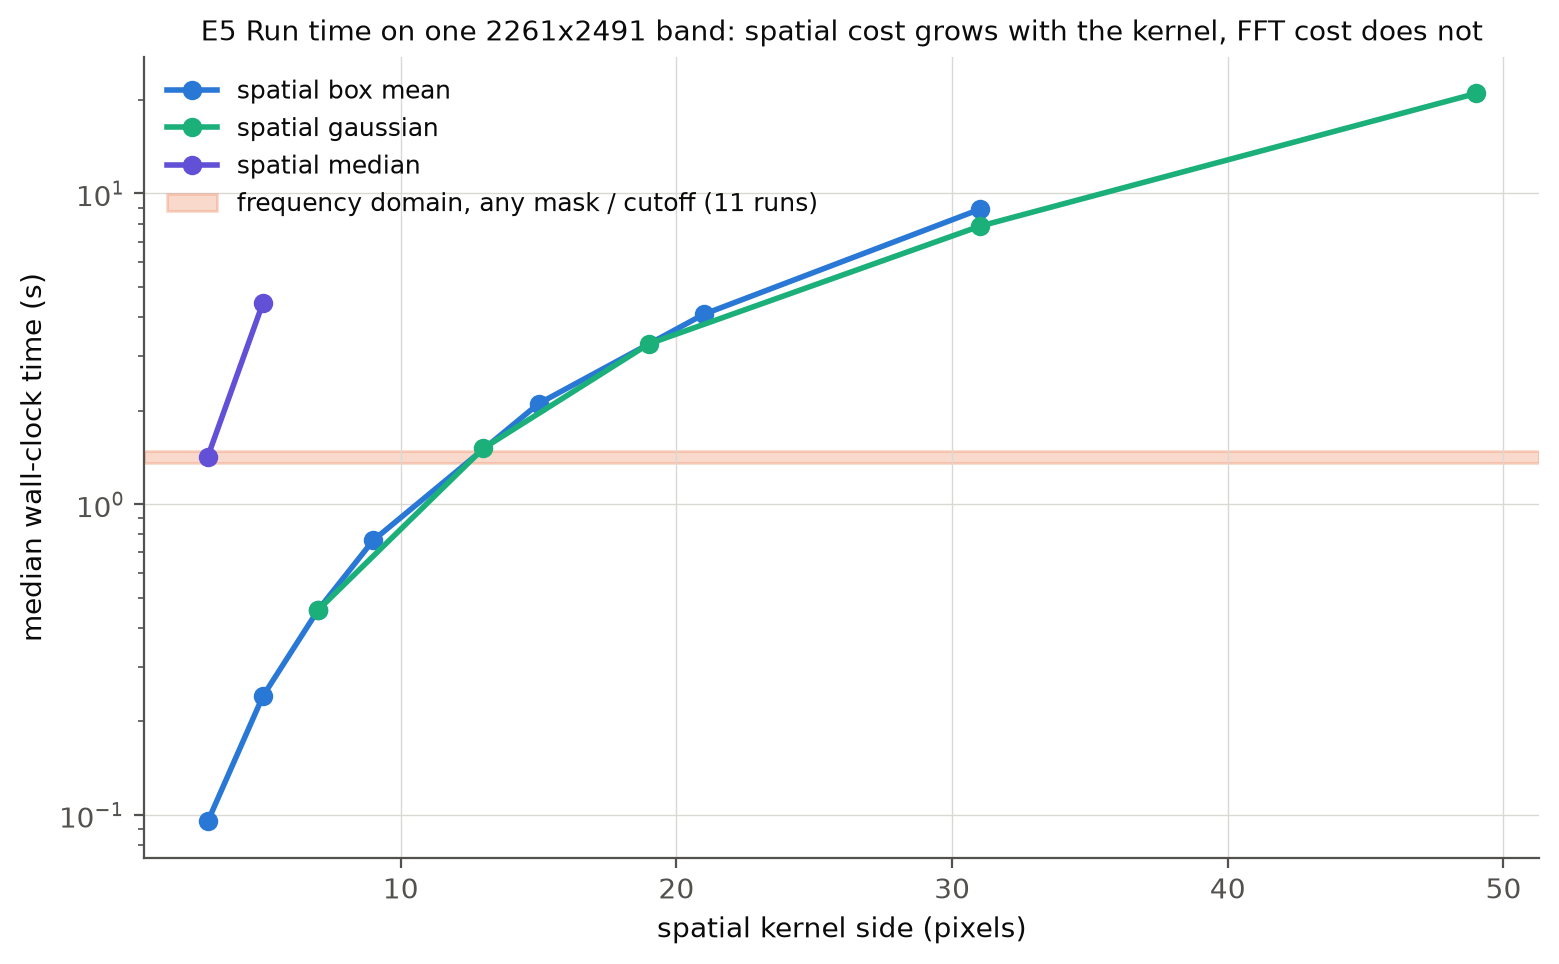
\includegraphics[width=\textwidth]{fig08_e5_runtime.png}
\column{0.40\textwidth}
\small
One full band, <<e5_shape>> px:
\begin{itemize}
\item Spatial mean $3\times3$: <<e5_box3>> s
\item Spatial mean $31\times31$: <<e5_box31>> s
\item Spatial Gaussian $49\times49$: <<e5_g8>> s
\item Any FFT mask: <<e5_fft_min>>--<<e5_fft_max>> s
\end{itemize}
Break-even near a <<e5_cross>>-px kernel
\end{columns}
\takeaway{\small Small kernels: convolve. Large kernels or many cutoffs: use the FFT.}
\end{frame}
\note{[Robin | 0:25 | 13:25]\\
Finally speed, on one full band. A 3 by 3 spatial filter took <<e5_box3>> seconds, but the time grows quickly with the kernel, up to <<e5_g8>> seconds for the largest. Every frequency-domain filter took about the same time, between <<e5_fft_min>> and <<e5_fft_max>> seconds, whatever the mask. The two lines cross near a kernel of <<e5_cross>> pixels. Since the filters that worked best are small, convolution is usually the practical choice. Sangeeta will bring the results together.}

% ================================================================== 6 Discussion and conclusions (Sangeeta)
\speaker{Sangeeta}
\section{Discussion and Conclusions}

\begin{frame}{Decision matrix: one best filter per application}
\centering
\footnotesize
\begin{tabular}{lll}
\toprule
Application & Best filter & Evidence (best vs.\ no filter) \\
\midrule
<<decision_table_slides>>
\bottomrule
\end{tabular}
\source{Generated by the analysis code from the experiment tables (\texttt{decision\_matrix.csv}).}
\takeaway{\small \textcolor{lpcol}{\textbf{Low-pass}} when pixel values feed a calculation;\quad \textcolor{hpcol}{\textbf{high-pass}} when edges and structure are the point.}
\end{frame}
\note{[Sangeeta | 0:35 | 14:00]\\
This table answers our five questions. It is produced by the code from the experiment results, with one measure per application. Some gains are large, like the median on impulse noise or the Gaussian for classification. Some are small, like urban boundaries and ridge coherence, and we present them as small. The pattern is consistent: low-pass filtering wins where pixel values feed a calculation, and high-pass filtering wins where the task is about where things change.}

\begin{frame}{Recommendation}
\begin{columns}[T, totalwidth=\textwidth]
\column{0.48\textwidth}
\begin{block}{Quantitative analysis}
\small
classification, indices, change detection\\[3pt]
$\Rightarrow$ light \textbf{Gaussian}, $\sigma\approx1.5$--2 px (or $D_0\approx0.2$)\\
$\Rightarrow$ \textbf{median $3\times3$} for impulse noise
\end{block}
\column{0.48\textwidth}
\begin{block}{Interpretation and mapping}
\small
visual analysis, boundaries, lineaments\\[3pt]
$\Rightarrow$ \textbf{high-boost}, $k=0.5$--1, for display\\
$\Rightarrow$ \textbf{Sobel / Prewitt} layer for lineaments
\end{block}
\end{columns}
\medskip
\begin{alertblock}{Avoid}
\small the ideal frequency mask (ringing), and heavy smoothing (detail is lost before noise)
\end{alertblock}
\end{frame}
\note{[Sangeeta | 0:30 | 14:30]\\
So our recommendation is split by purpose. For quantitative work, use light low-pass filtering: a small Gaussian, or a 3 by 3 median when there are dropped or saturated pixels. For interpretation and structural mapping, keep the original bands and add a high-pass product beside them: high-boost with moderate k for display, and a Sobel or Prewitt layer for lineaments. Avoid the ideal mask and avoid heavy smoothing.}

\begin{frame}{Limitations and conclusions}
\begin{columns}[T]
\column{0.50\textwidth}
\begin{block}{Limitations}
\footnotesize
\begin{itemize}
\item WorldCover is a model output, not ground truth
\item One winter scene, one area
\item One block split: $\kappa$ differences $\approx0.01$ are not a ranking
\item Coherence is a proxy for lineament quality
\item Bare/Mining (<<bare_pct>>\%): F1 $\le$ <<bare_f1_max>> for every input
\end{itemize}
\end{block}
\column{0.46\textwidth}
\begin{block}{Conclusions}
\footnotesize
\begin{itemize}
\item No single filter is ``most suitable''; the two families do opposite jobs
\item Smoothing: $\kappa$ +<<e2_kappa_gain>>, half the map speckle
\item Sharpening: best boundary match and sharpest image
\item Spatial and FFT routes agree for smooth masks
\end{itemize}
\end{block}
\end{columns}
\vfill
\centering
\large\textbf{Thank you. Questions?}\\[2pt]
\footnotesize Live demo: \texttt{python -m rsfilter demo} (offline, 512 $\times$ 512 sample)
\end{frame}
\note{[Sangeeta | 0:30 | 15:00]\\
Our results have limits. WorldCover is itself a model output; we used one winter scene and one area; and kappa differences of about 0.01 between the leading filters should not be read as a ranking. To conclude: there is no single most suitable filter, because the two families do opposite jobs. Smoothing gave the most accurate and cleanest land-cover map, and sharpening gave the best boundary match and the sharpest image. Thank you. We are happy to take questions, and we can run the offline demo if you would like to see it.}

% ------------------------------------------------------------------ references
\section*{References}
\begin{frame}[allowframebreaks]{References}
\nocite{*}
\tiny
\bibliographystyle{plainnat}
\bibliography{references}
\end{frame}

\end{document}
